%#########################################################################
\chapter{Oscilaciones}
\label{cha:oscillations}

El concepto de oscilación es ampliamente usado en ciencia y se aplica para
cualquier cantidad que presente fluctuaciones o perturbaciones en función 
del tiempo, ya sean periódicas o no. En este capítulo se presentan algunos
ejemplos de oscilaciones para sistemas mecánicos y electromagnéticos, que 
a pesar de su simplicidad, permiten ahondar en los detalles físicos de este
tipo de fenómenos.

\

La forma estándar de abordar un problema en una disciplina científica 
consiste en el estudio de situaciones ideales y muy particulares para llegar 
luego, usando refinamientos y consideraciones posteriores, a descripciones 
realistas y más generales. Por este motivo se comienza con demostraciones 
computacionales aplicadas a sistemas ideales, como el péndulo simple, el 
sistema masa resorte, etc. En demostraciones siguientes se abordarán 
aspectos cada vez más complejos de estos sistemas.
%#########################################################################



\
%*************************************************************************
\section{Demostración 1: Péndulo Simple Ideal}
\label{sec:DEMO2_01}
\rule{14cm}{0.5mm}

Como primer caso se aborda el péndulo simple. Este consiste en un sistema
de una masa $m$ con dimensión despreciable y bajo la acción de la 
gravedad $\bds g$, además pende de una cuerda tensa de longitud $l$ y sujeta
en un punto fijo. A partir de la figura \ref{fig:simple_pendulum}, la 
ecuación de movimiento está dada por


%.........................................................................
%Movement equation
\eq{eq:simple_pendulum}
{m\dtot{^2\bds r}{t^2} = m\bds g + \bds T}
%.........................................................................

\newpage
%.........................................................................
%Simple Pendulum
\begin{figure}[htbp]
	\centering
	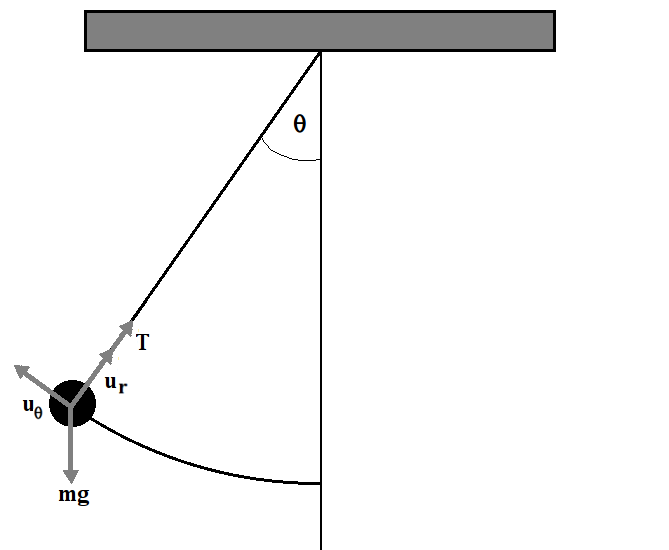
\includegraphics[width=0.50\textwidth]
	{./pictures/simple_pendulum.png}

	\caption{\small{Péndulo simple bajo la acción del campo gravitacional.}}
	
	\label{fig:simple_pendulum}
\end{figure}
%.........................................................................


En coordenadas polares se obtiene


%.........................................................................
%Movement equations
\begin{eqnarray}
\label{eq:simple_pendulum_1}
ml\dot \theta^2 &=& T - mg \cos \theta \\
\label{eq:simple_pendulum_2}
ml\ddot \theta &=& -mg \sin \theta
\end{eqnarray}
%.........................................................................


Como primera demostración computacional de este capítulo se solucionará el 
movimiento del péndulo simple a partir de las ecuaciones 
\ref{eq:simple_pendulum_1} y \ref{eq:simple_pendulum_2}. Para esto se 
asumirá que la amplitud de oscilación del péndulo es pequeña de tal forma 
que $\theta \approx \sin \theta$ y $\cos \theta \approx 1$, obteniendo


%.........................................................................
%Simplified equation
\eq{eq:simplified_pendulum}
{\ddot \theta = - \frac{g}{l} \theta}
%.........................................................................


Usando un ansatz de la forma $\theta(t) = e^{\lambda t}$ se llega a la
solución


%.........................................................................
%Approximate solution
\eq{eq:pendulum_solution}
{ \theta(t) = \theta_0 \sin ( \omega_0 t + \delta ) }
%.........................................................................
donde $\theta_0$ y $\delta$ son la amplitud y la fase respectivamente y 
constituyen las condiciones iniciales. La frecuencia $\omega_0$ está 
definida por 


%.........................................................................
%Frequancy
\eq{eq:freq_pedulum}
{ \omega_0 = \sqrt{ \frac{g}{l} } }
%.........................................................................

\

En el siguiente script de \python se grafica esta solución para diferentes
valores de la amplitud y la fase.

\newpage
%ccccccccccccccccccccccccccccccccccccccccccccccccccccccccccccccccccccccccc
%DEMO 2_01
\begin{listing}[style=python]
#!/usr/bin/env python
#==========================================================
# DEMOSTRACION 1
# Grafica de soluciones aproximadas del pendulo simple
#==========================================================
import numpy as np
import matplotlib.pylab as plt

#Solucion
def Theta(t):
    theta = theta0*np.sin( omega0*t + delta )
    return theta
    
#Gravedad
g = 9.8
#Longitud
l = 1
#Frecuencia
omega0 = np.sqrt( g/l )
#Tiempos
tiempo = np.arange( 0, 10, 0.1 )
    
#SOLUCION 1
#Amplitud
theta0 = 0.05
#Fase
delta = 0.0
#Grafica
plt.plot( tiempo, Theta(tiempo), label='solucion 1' )

#SOLUCION 2
#Amplitud
theta0 = 0.05
#Fase
delta = np.pi
#Grafica
plt.plot( tiempo, Theta(tiempo), label='solucion 2' )

#SOLUCION 3
#Amplitud
theta0 = 0.1
#Fase
delta = 0.0
#Grafica
plt.plot( tiempo, Theta(tiempo), label='solucion 3' )

plt.legend()
plt.show()
\end{listing}
%ccccccccccccccccccccccccccccccccccccccccccccccccccccccccccccccccccccccccc


El resultado que se obtiene es


%.........................................................................
%Simple Pendulum
\begin{figure}[htbp]
	\centering
	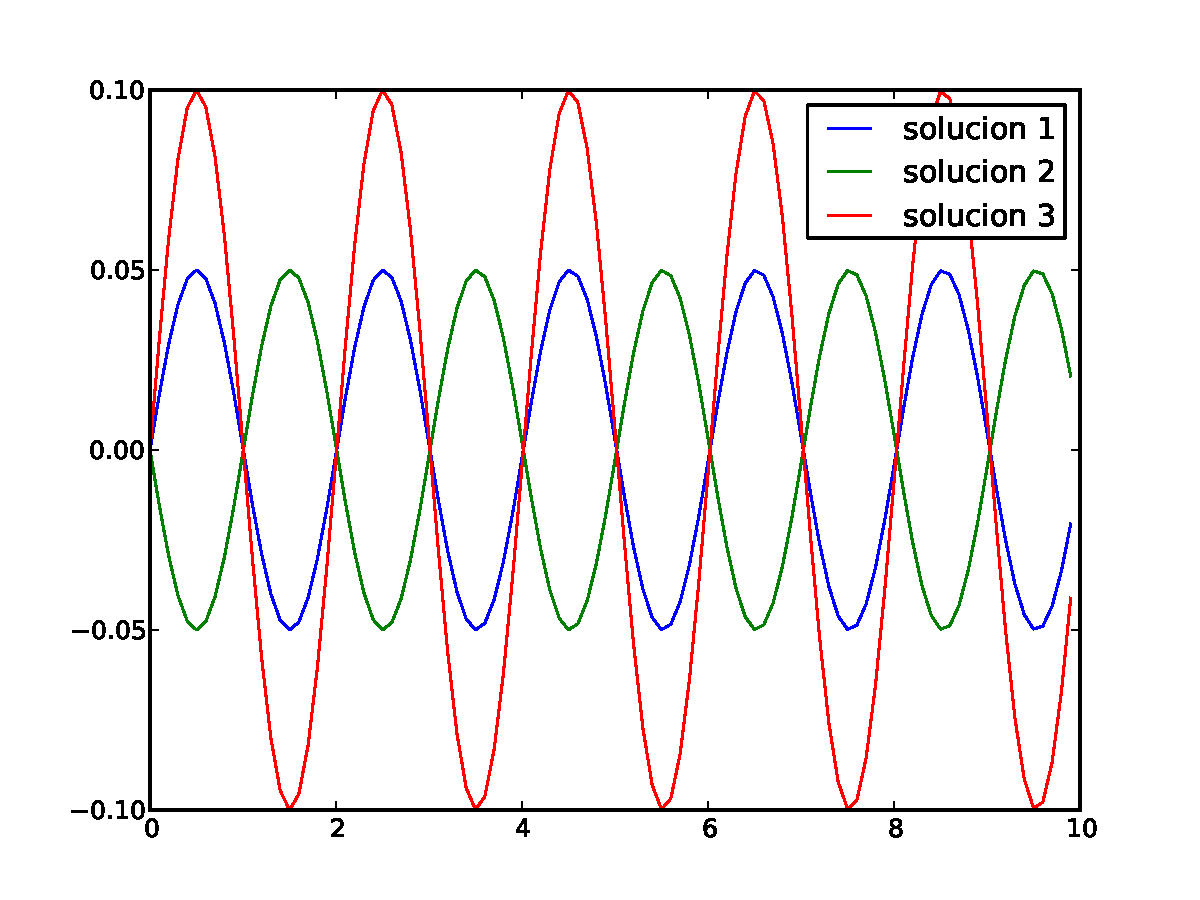
\includegraphics[width=0.8\textwidth]
	{./pictures/demo2_01.pdf}

	\caption{\small{Soluciones aproximadas obtenidas para el péndulo simple.}}
	
	\label{fig:approx_pedulum}
\end{figure}
%.........................................................................


En lo siguiente se explica cada porción de código.


%ccccccccccccccccccccccccccccccccccccccccccccccccccccccccccccccccccccccccc
%DEMO 2_01
\begin{listing}[style=python, numbers = none]
import numpy as np
import matplotlib.pylab as plt
\end{listing}
%ccccccccccccccccccccccccccccccccccccccccccccccccccccccccccccccccccccccccc
Esto corresponde al cargado de las librerías \numpy, bajo el alias de np y
\matplotlib bajo el alias de plt, ambas son necesarias para el desarrollo 
de todo el código.


%ccccccccccccccccccccccccccccccccccccccccccccccccccccccccccccccccccccccccc
%DEMO 2_01
\begin{listing}[style=python, numbers = none]
#Solucion
def Theta(t):
    theta = theta0*np.sin( omega0*t + delta )
    return theta
\end{listing}
%ccccccccccccccccccccccccccccccccccccccccccccccccccccccccccccccccccccccccc
En este parte se define la solución obtenida en la ecuación 
\ref{eq:pendulum_solution} para cualquier tiempo dado. Las funciones 
matemáticas estándar, tales como exponencial, logaritmo, trigonométricas, 
hiperbólicas, etc. Son accedidas desde el módulo \numpy como \texttt{np.sin},
\texttt{np.sinh}, \texttt{np.exp}, \texttt{np.log}, etc.


%ccccccccccccccccccccccccccccccccccccccccccccccccccccccccccccccccccccccccc
%DEMO 2_01
\begin{listing}[style=python, numbers = none]
#Gravedad
g = 9.8
#Longitud
l = 1
#Frecuencia
omega0 = np.sqrt( g/l )
#Tiempos
tiempo = np.arange( 0, 10, 0.1 )
\end{listing}
%ccccccccccccccccccccccccccccccccccccccccccccccccccccccccccccccccccccccccc
Se define la gravedad, la longitud de la cuerda (en metros), la frecuencia
de oscilación y finalmente, usando la función \texttt{arange} de la librería
\numpy, se cons\-truye un arreglo de tiempos donde es evaluada la solución, de 
0 a 10 segundos con saltos de 0.1.


%ccccccccccccccccccccccccccccccccccccccccccccccccccccccccccccccccccccccccc
%DEMO 2_01
\begin{listing}[style=python, numbers = none]
#SOLUCION 1
#Amplitud
theta0 = 0.05
#Fase
delta = 0.0
#Grafica
plt.plot( tiempo, Theta(tiempo), label='solucion 1' )
\end{listing}
%ccccccccccccccccccccccccccccccccccccccccccccccccccccccccccccccccccccccccc
La primera solución es obtenida para una amplitud de $\theta_0 = 0.05$ 
radianes y una fase $\delta = 0$. La última línea corresponde a la 
construcción de la gráfica de la solución. Para esto se usa la función 
\texttt{plot} de la librería \matplotlib. El primer argumento corresponde
a los datos asociados al eje x, en este caso \texttt{tiempo}, mientras el
segundo argumento son los datos asociados al eje y, en este caso la solución
evaluada en el tiempo, es decir \texttt{Theta(tiempo)}. El argumento 
\texttt{label} indica el nombre que tendrá la solución en la gráfica final,
esto se denomina etiqueta de la función.


%ccccccccccccccccccccccccccccccccccccccccccccccccccccccccccccccccccccccccc
%DEMO 2_01
\begin{listing}[style=python, numbers = none]
plt.legend()
plt.show()
\end{listing}
%ccccccccccccccccccccccccccccccccccccccccccccccccccccccccccccccccccccccccc
Finalmente se termina el script con la función \texttt{legend}, la cual 
muestra en pantalla las etiquetas puestas a cada gráfica. Y la función 
\texttt{show} que muestra en pantalla todas las soluciones.

\rule{14cm}{0.5mm}
%*************************************************************************



\
%*************************************************************************
\section{Demostración 2: Solución Exacta del Péndulo}
\label{sec:DEMO2_02}
\rule{14cm}{0.5mm}

La solución propuesta en la demostración anterior está basada en la 
aproximación de pequeñas oscilaciones, para la cual $\sin \theta \approx 
\theta$ y $\cos \theta \approx 1$, aún así, a medida que el movimiento sea
de mayor amplitud, esta aproximación deja de ser válida y se la solución 
general debe obtenerse directamente de las ecuaciones 
\ref{eq:simple_pendulum_1} y \ref{eq:simple_pendulum_2}

\

Una forma conveniente de reescribir las ecuaciones de movimiento es derivando
\ref{eq:simple_pendulum_1} respecto al tiempo e introduciendo la ecuación
\ref{eq:simple_pendulum_2}


%.........................................................................
%Tension
\begin{eqnarray}
\nonumber
\dot T &=& \dot \theta \pr{ 2ml\ddot \theta - mg\sin \theta } \\
\nonumber
\dot T &=& -\dot \theta \pr{ 2mg\sin \theta + mg\sin \theta } \\
\label{eq:new_tension}
\dot T &=& -3\dot \theta mg\sin \theta
\end{eqnarray}
%.........................................................................


Definiendo la velocidad angular $\omega = \dot \theta$, el sistema de 
ecuaciones originales junto con la ecuación \ref{eq:new_tension} queda


%.........................................................................
%Tension
\begin{eqnarray}
\label{eq:Dtheta}
\dot \theta &=& \omega \\
\label{eq:Domega}
\dot \omega &=& -\frac{g}{l}\sin \theta \\
\label{eq:Dtension}
\dot T &=& -3\omega mg\sin \theta
\end{eqnarray}
%.........................................................................


Esta forma se denomina sistema de ecuaciones diferenciales lineales y es 
esencial para la solución exacta a partir de algoritmos de integración 
numérica.

\

Las condiciones iniciales para la solución aproximada son completamente 
determinadas a partir de la fase $\delta$ y la amplitud $\theta_0$. En el 
caso de la solución exacta es necesario suministrar tres condiciones para
cada una de las variables de las ecuaciones \ref{eq:Dtheta} - 
\ref{eq:Dtension}, es decir, la posición angular inicial del péndulo 
$\theta_{t_0}$, la velocidad angular inicial $\omega_{t_0}$ y la tensión
inicial $T_{t_0}$. Aún así, la tensión inicial depende de las otras dos 
condiciones a través de la ecuación \ref{eq:simple_pendulum_1}


%.........................................................................
%T0_equation
\eq{eq:initial_tension}
{T_{t_0} = ml\omega_{t_0}^2 + mg \cos \theta_{t_0}}
%.........................................................................


En esta demostración se calcularán ambas soluciones para un péndulo con 
condiciones iniciales fijadas. La solución numérica se realiza a partir del
la rutina de integración numérica \texttt{odeint} del módulo \texttt{integrate}
del paquete \scipy.


%ccccccccccccccccccccccccccccccccccccccccccccccccccccccccccccccccccccccccc
%DEMO 2_02
\begin{listing}[style=python]
#!/usr/bin/env python
#==========================================================
# DEMOSTRACION 2
# Comparacion de solucion completa y aproximada para el 
# pendulo simple
#==========================================================
import numpy as np
import matplotlib.pylab as plt
import scipy.integrate as integ

#Solucion aproximada
def Theta(t):
    theta = theta0*np.sin( omega0*t + delta )
    return theta

#Ecuaciones de movimiento
def dF(Y, t):
    #Valor anterior de theta
    theta = Y[0]
    #Valor anterior de omega
    omega = Y[1]
    #Valor anterior de la tension
    tension = Y[2]
    #Derivada de theta
    Dtheta = omega
    #Derivada de omega
    Domega = -g*np.sin( theta )/l
    #Derivada de la tension
    Dtension = -3*omega**m*g*np.sin( theta )
    return (Dtheta, Domega, Dtension)
    
#Gravedad
g = 9.8
#Longitud
l = 1
#Masa
m = 1
#Frecuencia
omega0 = np.sqrt( g/l )
#Tiempos
tiempo = np.arange( 0, 10, 0.01 )
    
#SOLUCION APROXIMADA
#Amplitud
theta0 = np.pi/4
#Fase
delta = np.pi/2.
#Grafica
plt.plot(tiempo, Theta(tiempo), label='solucion aproximada')

#SOLUCION NUMERICA
#Angulo inicial
theta_t0 = np.pi/4
#Velocidad angular inicial
omega_t0 = 0.0
#Tension inicial
tension_t0 = m*l*omega_t0**2 + m*g*np.cos( theta_t0 )
#Condiciones iniciales
cond_ini = ( theta_t0, omega_t0, tension_t0 )
#Solucion numerica
theta_t, omega_t, tension_t = np.transpose( 
integ.odeint( dF, cond_ini, tiempo ) )
#Grafica
plt.plot( tiempo, theta_t, label='solucion numerica' )

plt.legend()
plt.show()
\end{listing}
%ccccccccccccccccccccccccccccccccccccccccccccccccccccccccccccccccccccccccc

\

Para ambas soluciones se ha asumido una amplitud de $\theta_0 = 45^o = 
\pi/4$ y las condiciones iniciales son definidas de tal forma que el 
péndulo sea soltado desde su máxima amplitud. En el caso de la solución 
aproximada, esto implica una amplitud $\theta_0 = \pi/4$ y una fase de 
$\delta = \pi/2$. Para la solución aproximada, las condiciones equivalentes 
son $\theta_{t_0} = \pi/4$ y $\omega_{t_0} = 0$. El resultado de la 
integración para 10 segundos es mostrado en la figura 
\ref{fig:numeric_pedulum}.

\

Cambiando la amplitud inicial a un valor $\theta = 10^o \approx 0.17$ 
ambas soluciones son muy similares, indicando el rango de la validez de 
la aproximación inicial. El resultado para 10 segundos es mostrado en la 
figura \ref{fig:small_pedulum}.


%.........................................................................
%Simple Pendulum Exact solution
\begin{figure}[htbp]
	\centering
	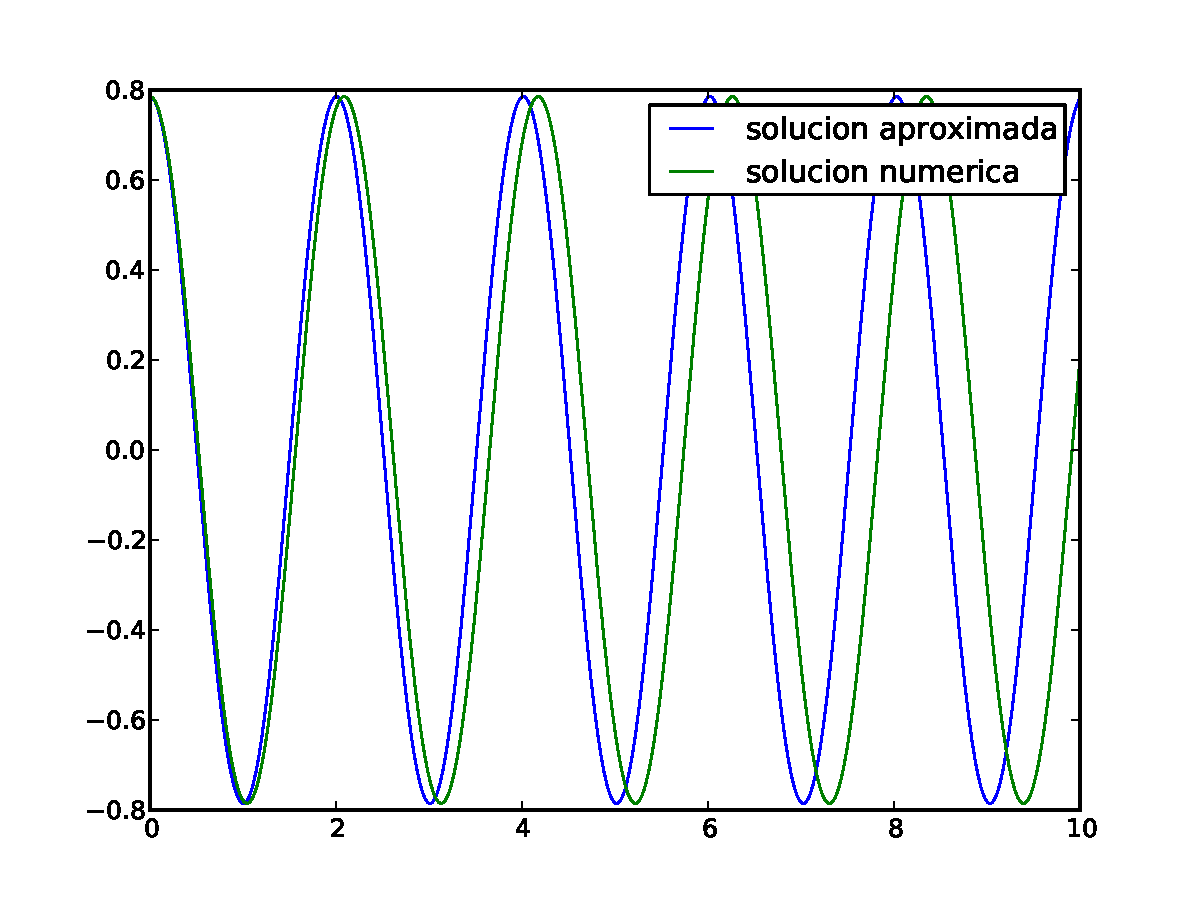
\includegraphics[width=0.80\textwidth]
	{./pictures/demo2_02.pdf}

	\caption{\small{Comparación entre la solución exacta numérica y la 
	solución aproximada. Debido a la mayor amplitud de oscilación, la 
	aproximación de pequeñas oscilaciones deja de ser válida y difiere 
	considerablemente de la solución real.}}
	
	\label{fig:numeric_pedulum}
\end{figure}
%.........................................................................


%.........................................................................
%Simple Pendulum Exact solution
\begin{figure}[htbp]
	\centering
	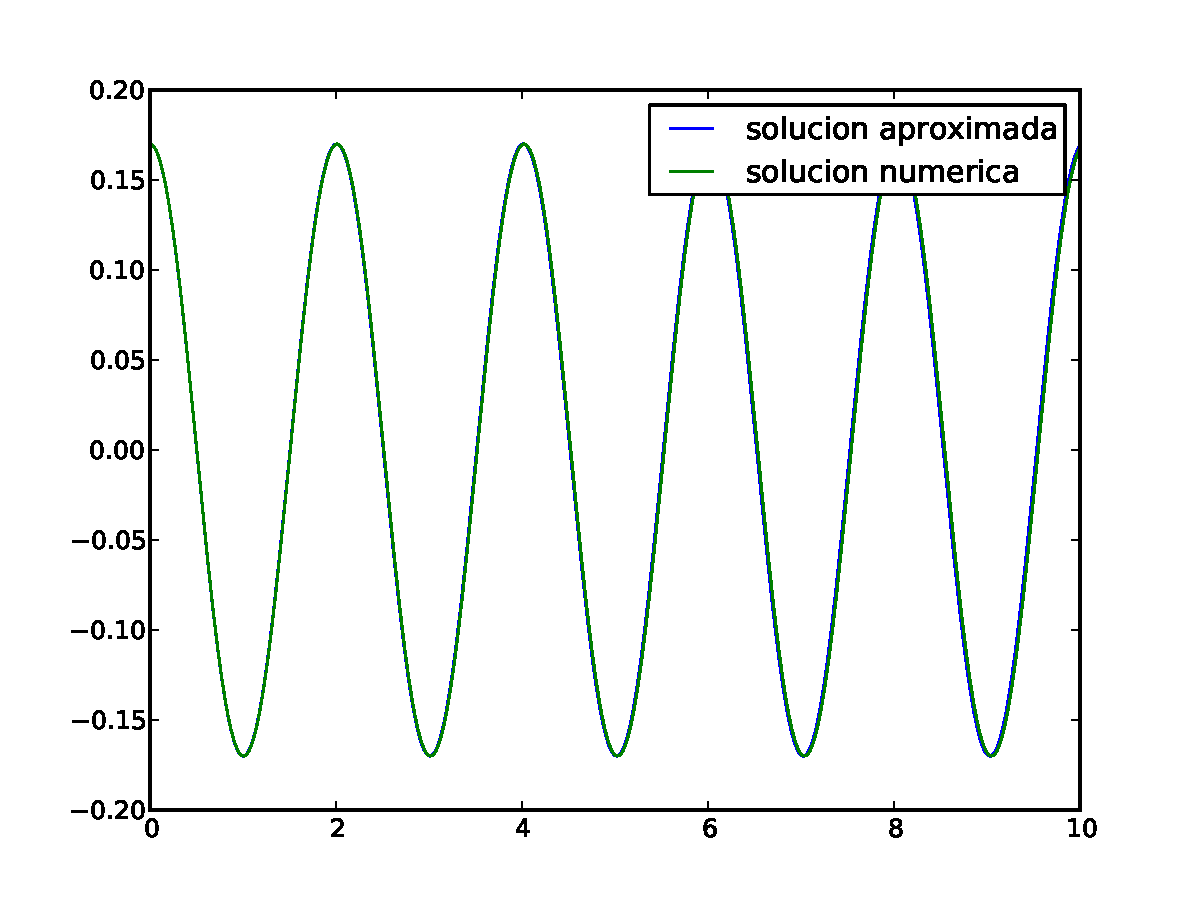
\includegraphics[width=0.80\textwidth]
	{./pictures/demo2_02(02).pdf}

	\caption{\small{Comparación entre la solución exacta numérica y la 
	solución aproximada. Para pequeñas amplitudes ambas soluciones son
	muy similares.}}
	
	\label{fig:small_pedulum}
\end{figure}
%.........................................................................
\newpage

A continuación se explican las nuevas partes introducidas en el código en 
comparación con la demostración 1.


%ccccccccccccccccccccccccccccccccccccccccccccccccccccccccccccccccccccccccc
%DEMO 2_02
\begin{listing}[style=python, numbers = none]
import scipy.integrate as integ
\end{listing}
%ccccccccccccccccccccccccccccccccccccccccccccccccccccccccccccccccccccccccc
Esto corresponde al cargado del módulo \texttt{integrate} de \scipy bajo el
alias de \texttt{integ} para las funcionalidades de integración numérica.


%ccccccccccccccccccccccccccccccccccccccccccccccccccccccccccccccccccccccccc
%DEMO 2_02
\begin{listing}[style=python, numbers = none]
#Ecuaciones de movimiento
def dF(Y, t):
    #Valor anterior de theta
    theta = Y[0]
    #Valor anterior de omega
    omega = Y[1]
    #Valor anterior de la tension
    tension = Y[2]
    #Derivada de theta
    Dtheta = omega
    #Derivada de omega
    Domega = -g*np.sin( theta )/l
    #Derivada de la tension
    Dtension = -3*omega**m*g*np.sin( theta )
    return (Dtheta, Domega, Dtension)
\end{listing}
%ccccccccccccccccccccccccccccccccccccccccccccccccccccccccccccccccccccccccc
Se define la función que contiene las derivadas de cada una de las 
variables del sistema, acorde al sistema \ref{eq:Dtheta} - \ref{eq:Dtension}.
\texttt{Y} es un arreglo que contiene las variables $\theta$, $\omega$ y $T$
en el tiempo anterior respectivamente y \texttt{t} el tiempo actual.


%ccccccccccccccccccccccccccccccccccccccccccccccccccccccccccccccccccccccccc
%DEMO 2_02
\begin{listing}[style=python, numbers = none]
#SOLUCION NUMERICA
#Angulo inicial
theta_t0 = np.pi/4
#Velocidad angular inicial
omega_t0 = 0.0
#Tension inicial
tension_t0 = m*l*omega_t0**2 + m*g*np.cos( theta_t0 )
#Condiciones iniciales
cond_ini = ( theta_t0, omega_t0, tension_t0 )
#Solucion numerica
theta_t, omega_t, tension_t = np.transpose( 
integ.odeint( dF, cond_ini, tiempo ) )
#Grafica
plt.plot( tiempo, theta_t, label='solucion numerica' )
\end{listing}
%ccccccccccccccccccccccccccccccccccccccccccccccccccccccccccccccccccccccccc
Finalmente se realiza la integración de la solución exacta del péndulo 
simple. Se dan las condiciones iniciales para el ángulo y la velocidad 
angular inicial, para la tensión se usa la ecuación \ref{eq:initial_tension}.
Luego, en un arreglo \texttt{cond\_ini} se ponen las tres condiciones para 
luego llamar la función \texttt{integ.odeint}. Esta tiene como primer 
argumento la función \texttt{dF} con las ecuaciones de movimiento del 
sistema, segundo argumento el arreglo de condiciones iniciales y 
como tercero el arreglo de tiempo donde se desea evaluar la solución.
Finalmente se grafica la solución.

\rule{14cm}{0.5mm}
%*************************************************************************